\documentclass{article} 
\usepackage[utf8]{inputenc}
\usepackage{amsmath, amssymb, systeme, mathtools, lmodern, float, graphicx, titlesec}
\usepackage[most]{tcolorbox}
\usepackage[scale=.95,type1]{cabin}
\usepackage[framemethod=tikz]{mdframed}


\usepackage[legalpaper,margin=1in]{geometry}

\setlength{\parindent}{10pt}
\setlength{\parskip}{1em}
\renewcommand{\baselinestretch}{1.2}

\title{PARTIAL DERIVATIVES}
\date{}
\author{}

\makeatletter
\renewcommand*\env@matrix[1][*\c@MaxMatrixCols c]{%
  \hskip -\arraycolsep
  \let\@ifnextchar\new@ifnextchar
  \array{#1}}
\makeatother

\DeclarePairedDelimiter\abs{\lvert}{\rvert}
\DeclarePairedDelimiter\norm{\lVert}{\rVert}
\makeatletter 
\let\oldabs\abs
\def\abs{\@ifstar{\oldabs}{\oldabs*}}

\let\oldnorm\norm
\def\norm{\@ifstar{\oldnorm}{\oldnorm*}}
\makeatother

\newcommand\y{\cellcolor{blue!10}}

\usepackage{tabularray}
\SetTblrInner{colsep=5pt,rowsep=1pt}

\newcounter{Def}[section]
\newenvironment{Def}[1][]{%
  \ifstrempty{#1}%
  {\mdfsetup{%
    frametitle={%
      \tikz[baseline=(current bounding box.east),outer sep=0pt]
      \node[line width=1pt,anchor=east,rectangle,draw=blue!20,fill=white]
    {\strut \color{black}{Definition}~};}}
  }%
  {\mdfsetup{%
    frametitle={%
      \tikz[baseline=(current bounding box.east),outer sep=0pt]
      \node[line width=1pt,anchor=east,rectangle,draw=blue!20,fill=white]
    {\strut \color{black}{Definition}~:~\color{blue4}{#1}};}}%
  }%
  \mdfsetup{innertopmargin=2pt,linecolor=blue!20,%
            linewidth=1pt,topline=true,%
            frametitleaboveskip=\dimexpr-\ht\strutbox\relax,}
  \begin{mdframed}[]\relax%
  }{\end{mdframed}}
%{\fontfamily{cmtt}\selectfont }
\titleformat{\section}
  {\fontfamily{lmss}\selectfont\LARGE\bfseries\color{black}}
  {\thesection}{1em}{}
\begin{document}
\mdfdefinestyle{MyFrame}{%
    linecolor=black,
    outerlinewidth=2pt,
    %roundcorner=20pt,
    innertopmargin=4pt,
    innerbottommargin=4pt,
    innerrightmargin=4pt,
    innerleftmargin=4pt,
        leftmargin = 4pt,
        rightmargin = 4pt
    %backgroundcolor=gray!50!white}
        }

\section{Functions of Several Variables}
\subsection*{{\fontfamily{lmss}\selectfont \underline{Functions of Two Variables}}}
\begin{Def}[]
  A \textbf{function $f$ of two variables} is a rule that assigns to each ordered pair of real numbers $(x,y)$ in a set $D$ (domain  subset of $\mathbb{R}^2$) of $f(x,y)$ (range subset of $\mathbb{R}$). 
\end{Def}

\begin{minipage}[]{0.34\linewidth}
  \begin{center}
    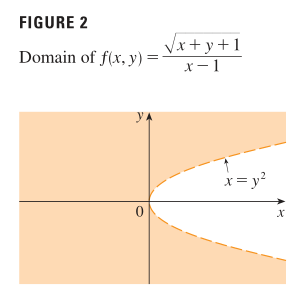
\includegraphics[width = 4.8 cm]{./images/eg1.png} 
  \end{center}
\end{minipage}
\begin{minipage}[]{0.6\linewidth}
{\fontfamily{lmtt}\selectfont \textbf{\textcolor{blue5}{EXAMPLE.}}} 

Evaluate $f(3,2)$,  find and sketch the domain of $f(x,y) = \ln{(y^2 - x)}$.
\[f(3,2) = 3 \ln{(2^2 - 3)} = 3 \ln{1} = 0\]
The domain of $f$ is $D = \{(x, y) \text{ } | \text{ } x < y^2\}$.
\end{minipage}
\subsection*{{\fontfamily{lmss}\selectfont \underline{Graph}}}
\begin{minipage}[]{0.3\linewidth}
  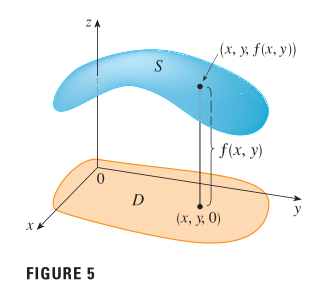
\includegraphics[width = 4 cm]{./images/graph.png}
\end{minipage}
\begin{minipage}[]{0.6\linewidth}
  The graph of $f(x,y)$ is the set of all points $(x,y,z)$ in $\mathbb{R}^3$.
\end{minipage}

{\fontfamily{lmtt}\selectfont \textbf{\textcolor{blue5}{EXAMPLE.}}} Sketch the graph of $f(x,y) = 6 - 3x - 2y$.

\begin{minipage}[]{0.3\linewidth}
  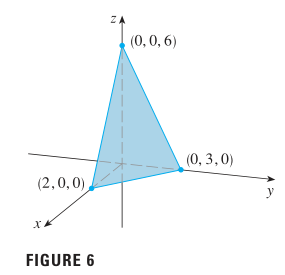
\includegraphics[width = 4 cm]{./images/eg5.png}
  
\end{minipage}
\begin{minipage}[]{0.6\linewidth}
  {\fontfamily{lmtt}\selectfont \textbf{\textcolor{blue5}{A linear function...}}} 

  The equation of the graph is $3x + 2 + z = 6$, which represents a plane. To graph it, find the \textit{intercepts} by setting 2 of the 3 variables to 0.
\end{minipage}

{\fontfamily{lmtt}\selectfont \textbf{\textcolor{blue5}{EXAMPLE.}}} Sketch the graph of $g(x,y) = \sqrt{9 - x^2 - y^2}$.

\begin{minipage}[]{0.34\linewidth}
  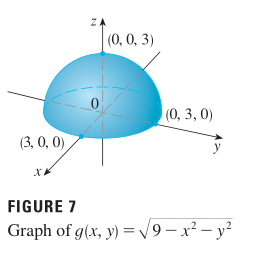
\includegraphics[width = 4 cm]{./images/eg6.png}
  
\end{minipage}
\begin{minipage}[]{0.6\linewidth}
  Square both sides of this equation to obtain $x^2 + y^2 + z^2 = 9$.

  Since $z \ge 0$, this is the upper part of a sphere whose center the origin and radius 3.
\end{minipage}

\pagebreak
Computer programs can graph functions $f(x,y)$. Traces in the vertical planes $x = k$ and $y = k$ are drawn for equally spaced values of $k$ and parts of the graph are eliminated using hidden line removal.
\begin{center}
  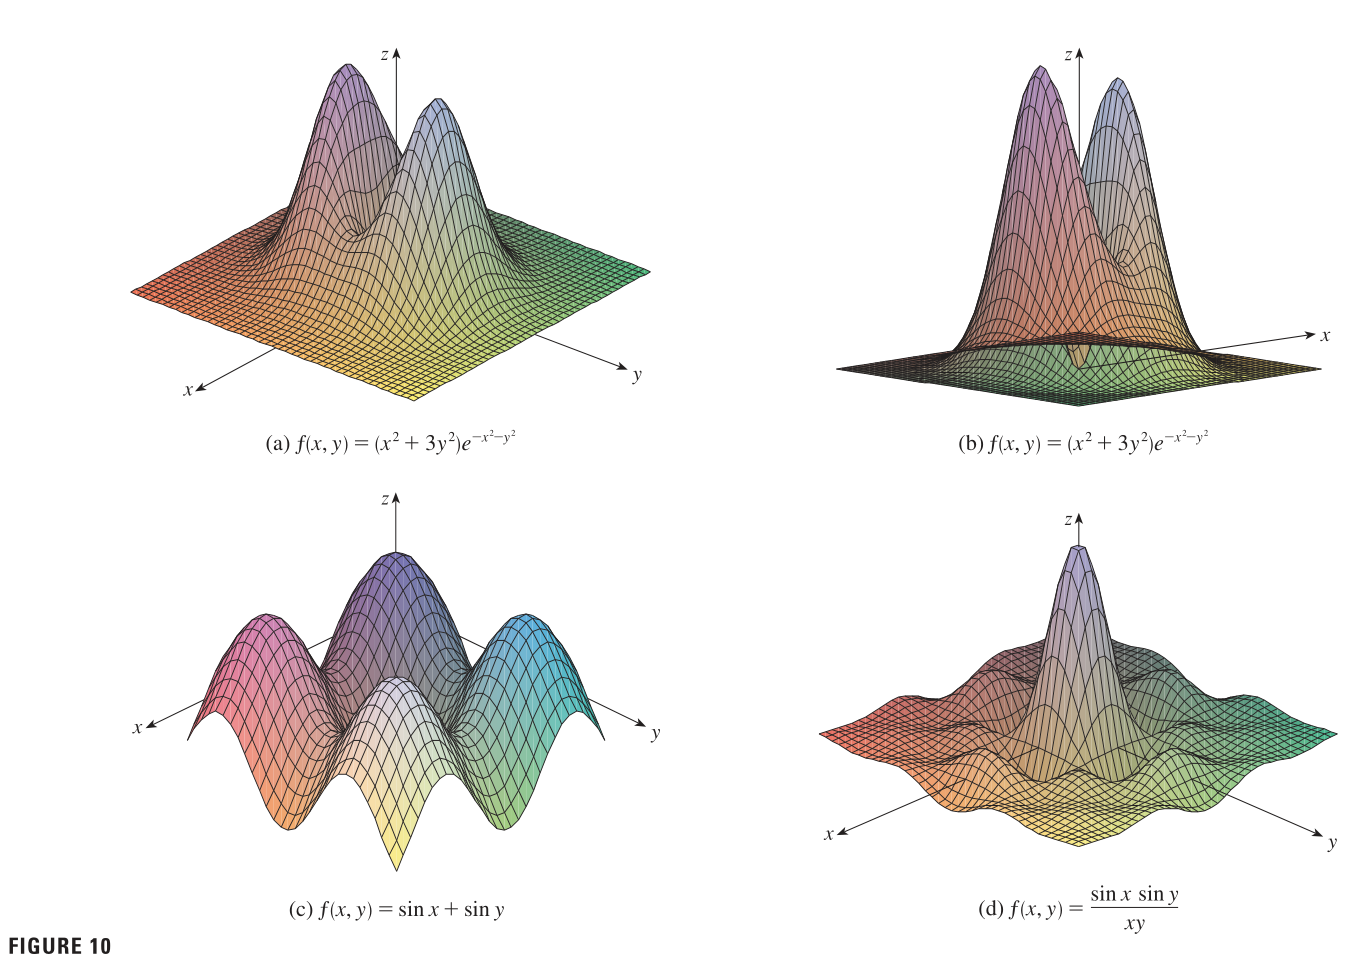
\includegraphics[width = 15 cm]{./images/blender.png} 
\end{center}

\subsection*{{\fontfamily{lmss}\selectfont \underline{Level Curves}}}
Beside arrow diagrams and graphs, we visualize a function using \textit{level curves}, or \textit{contour lines}, formed by a contour map on which points of constant elevation are joined.
\begin{center}
  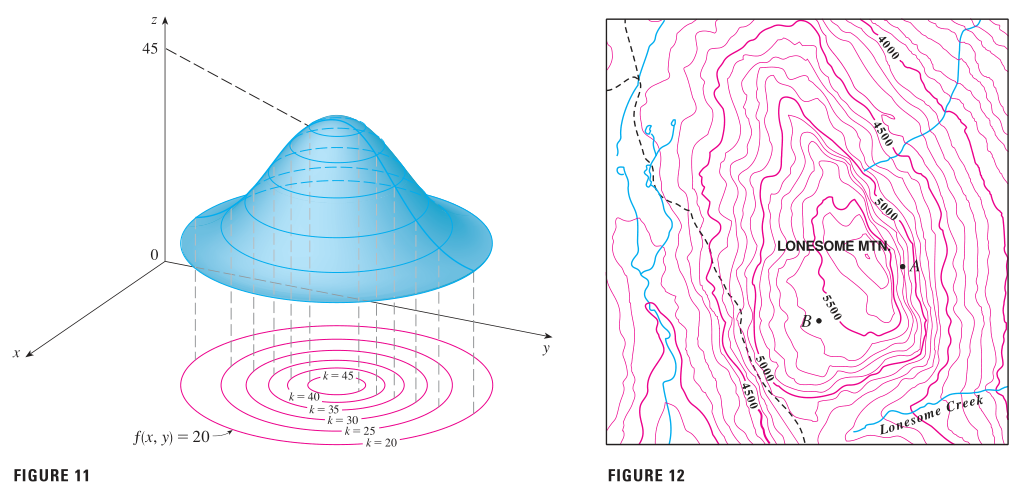
\includegraphics[width = 15 cm]{./images/contour.png} 
\end{center}
Another example of the temperature functions, the level curves are \textbf{isothermals}.
\begin{center}
  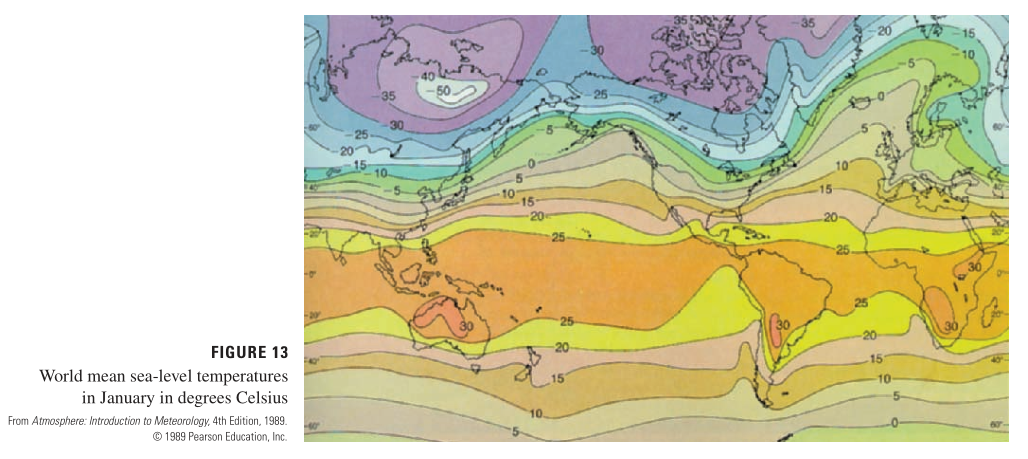
\includegraphics[width = 13.1 cm]{./images/temperature.png} 
\end{center}

For some purpuses, a contour map is more useful than a graph.
\begin{center}
  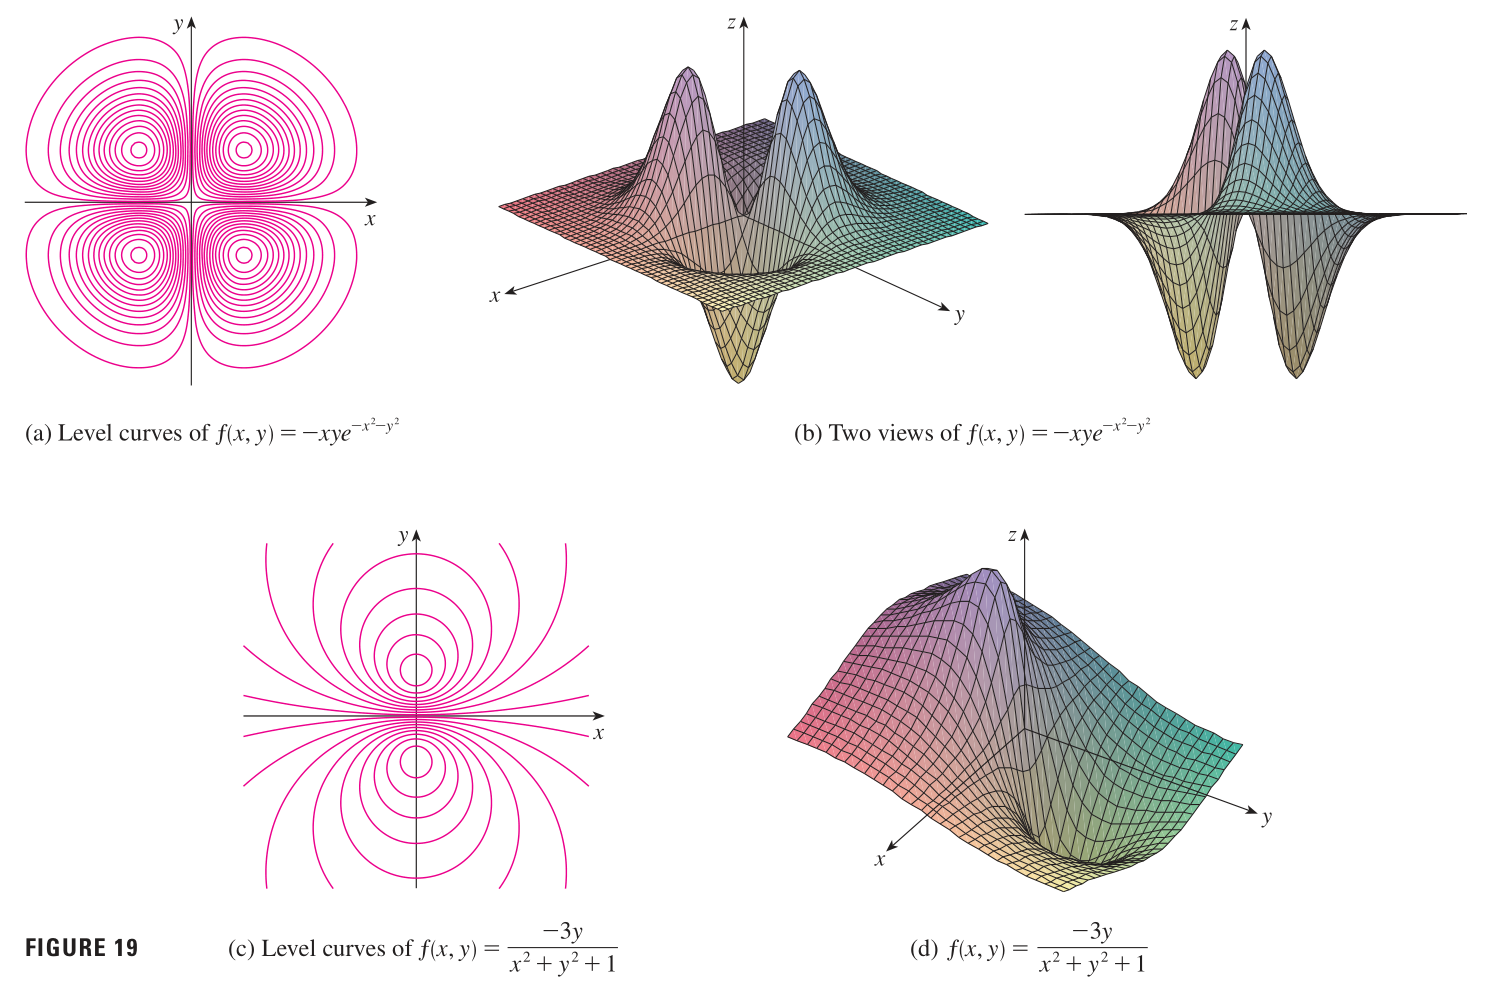
\includegraphics[width = 16 cm]{./images/levelcurves.png} 
\end{center}

\subsection*{{\fontfamily{lmss}\selectfont \underline{Functions of Three or More Variables}}}
It's hard to visualize $f(x,y,z)$ by its graph (four-dimensional space). We examine its \textbf{level surfaces}, which are the surfaces of $f(x,y,z) = k$.

{\fontfamily{lmtt}\selectfont \textbf{\textcolor{blue5}{EXAMPLE.}}} Find the level surfaces of  $f(x,y,z) = x^2 + y^2 + z^2 $.

\begin{minipage}[]{0.35\linewidth}
\begin{center}
  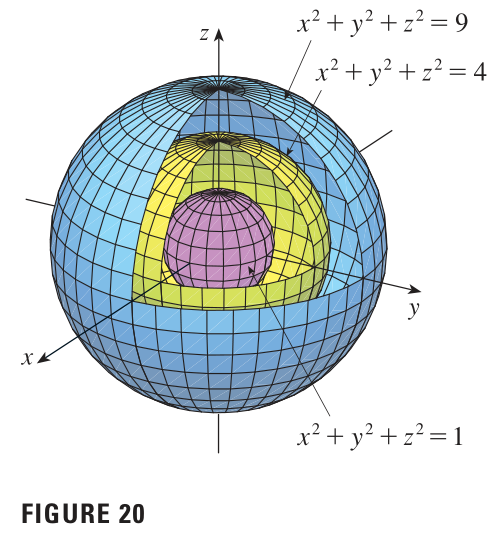
\includegraphics[width = 5 cm]{./images/eg15.png} 
\end{center}
  
\end{minipage}
\begin{minipage}[]{0.6\linewidth}
  The level surfaces are $x^2 + y^2 + z^2 = k \ge 0$, which forms a family of concentric spheres with radius $\sqrt{k}$.
\end{minipage}

\begin{Def}[]
  A \textbf{function of n variables} is a rule that assigns a number $z = f(x_1, x_2 , \dots , x_n)$ to an $n$-tuple $(x_1, x_2, \dots, x_n)$. The set of all $n$-tuples is $\mathbb{R}^n$. We can look at it as a function of
  \begin{itemize}
    \item $n$ real variables $x_1, x_2, \dots, x_n$.
    \item A single point $(x_1, x_2, \dots, x_n)$.
    \item A single vector $\textbf{x} = \langle x_1, x_2, \dots, x_n \rangle$
  \end{itemize}
\end{Def}
\pagebreak
\section{Limits and Continuity}
Let's compare 2 functions as $(x,y)$ approach the origin.
\[f(x,y) = \frac{\sin{x^2 + y^2 }}{x^2 + y^2 }   \quad \text{and} \quad g(x,y)= \frac{x^2 - y^2 }{x^2 + y^2 }\]
\begin{center}
  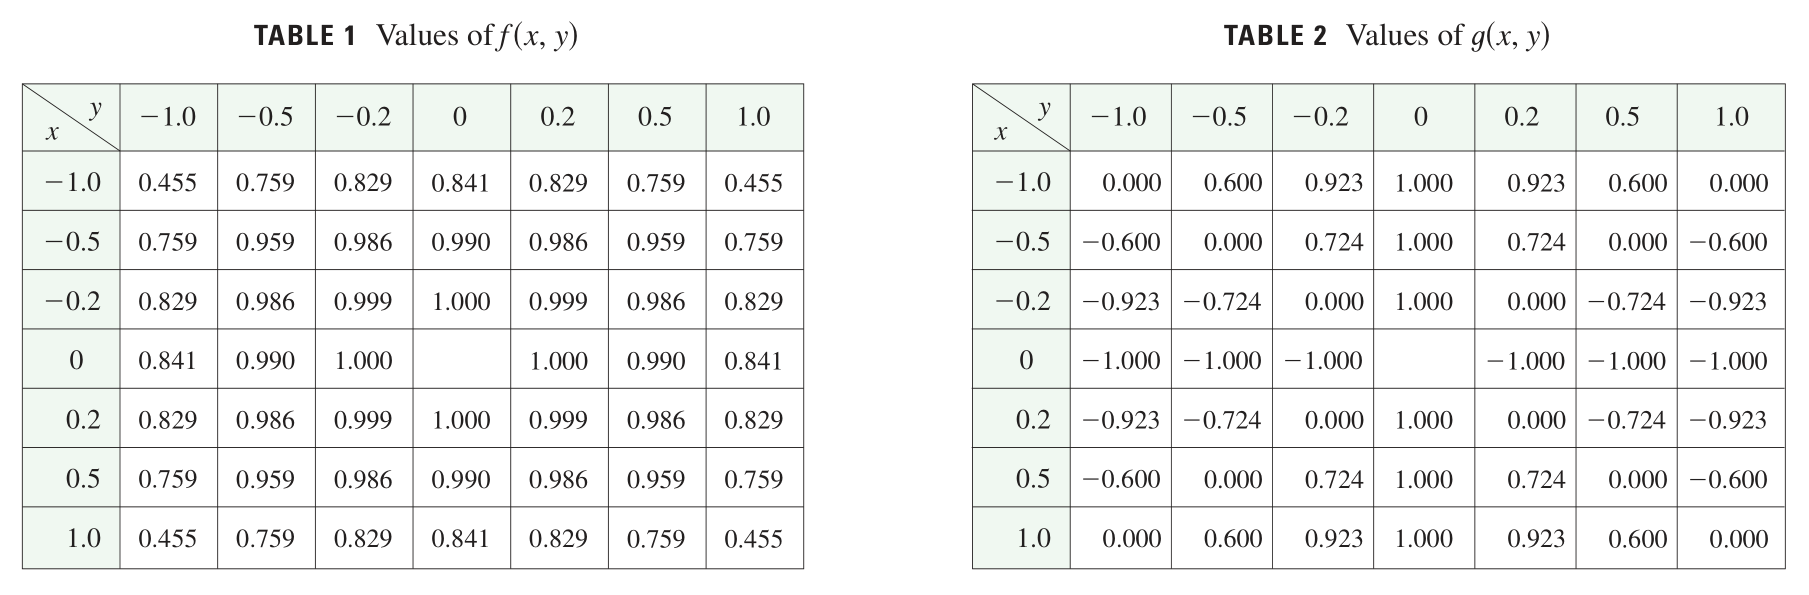
\includegraphics[width = 15 cm]{./images/cmpFG.png}
\end{center}
It appears that $f(x,y)$ are approaching 1 whereas $g(x,y)$ aren't approaching any number.
\begin{Def}[Limit]
The domain $D$ includes points arbitrarily close to $(a,b)$.
 The \textbf{limit of $f(x,y)$ as $(x,y)$ approaches $(a,b)$} is $L$. 
 \[\lim_{(x,y) \to (a,b)} f(x,y) = L\]
 if for $\forall \varepsilon > 0$, there is a corresponding $\delta > 0$ such that 
 \begin{center}
   if $(x,y) \in D$ and $0 < \sqrt{(x - a)^2 + (y - b)^2 } < \delta$ then 
   $f(x,y) - L| < \varepsilon$    
 \end{center}

\end{Def}
   {\fontfamily{lmtt}\selectfont \textbf{\textcolor{blue5}{Note.}}} $|f(x,y) - L|$ is the distance between $f(x,y)$ and $L$. 

   $\quad \sqrt{(x-a)^2 + (y-b)^2}$ is the distance between the  point $(x,y)$ and $(a,b)$ .

  If $(L - \varepsilon, L + \varepsilon     )$ is given, we can find a disk $D_\delta$ with a center $(a,b)$ and radius $\delta > 0$ such that $f$ maps all the points in $D_\delta$ (except possibly $(a,b)$) into $(L - \varepsilon, L + \varepsilon     )$.
  \begin{center}
    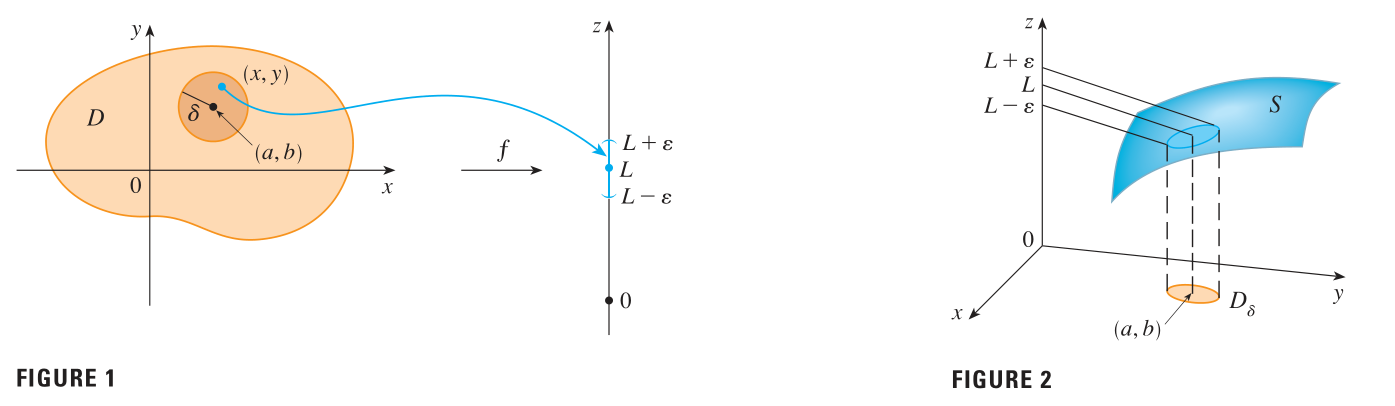
\includegraphics[width = 15 cm]{./images/limit.png} 
  \end{center}
  
  \textbf{1 variable.}   Recall that for $f(x)$, there are only 2 directions of approach, from the left \textit{or} from the right. And if $\lim_{x \to a^{-}} f(x) \ne \lim_{x \to a^{+}} f(x)$, then $lim_{x \to a} f(x)$ does not exist.

  \textbf{2 variables.} We can't just let $(x,y)$ approach $(a,b)$ from an infinite number of directions. But if the limit exists, the $f(x,y)$ must approach the \textbf{same limit} no matter how. 
  \begin{mdframed}
    If $f(x,y) \to L_1$ as $(x,y) \to (a,b)$ along a path $C_1$ and $f(x,y) \to L_2$ as $(x,y) \to (a,b)$ along a path $C_2$, where $L_1 \ne L_2$, then $\lim_{(x,y) \to (a,b)} f(x,y)$ does not exist.
  \end{mdframed}
  {\fontfamily{lmtt}\selectfont \textbf{\textcolor{blue5}{EXAMPLE.}}} Show that  this does not exist \[\lim_{(x,y) \to (0,0)} \frac{x^2 - y^2 }{x^2 + y^2 }\]

  \begin{minipage}[]{0.35\textwidth}
    \begin{center}
      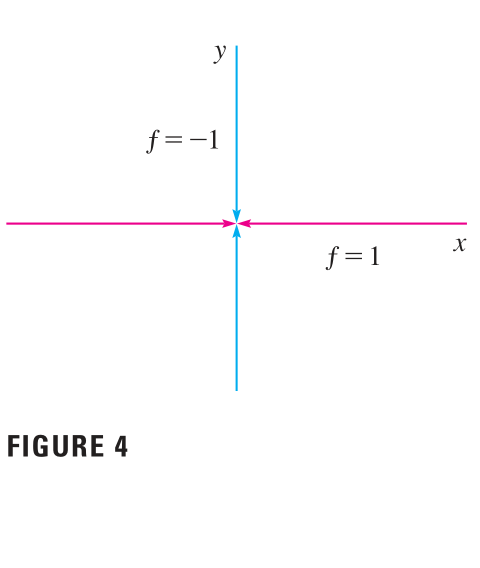
\includegraphics[width = 5 cm]{./images/limeg1.png} 
    \end{center}
  \end{minipage}
  \begin{minipage}[]{0.6\textwidth}
    Let $f(x,y) = (x^2 - y^2 )/(x^2 + y^2 )$. \\ $\square$ First, let approach $(0,0)$ along the $x$-axis.\\
    Then $\quad y = 0$ gives $f(x,0) = x^2 / x^2 = 1$ for $\forall x \ne 0$.
    \begin{center}
    $f(x,y) \to 1  \quad \text{as} \quad (x,y) \to (0,0)$ along the $x$-axis
    \end{center}  
    $\square$ Now, approach along the $y$-axis by putting $x = 0$.\\
    Then $\quad f(0,y) = -y^2 / y^2 = -1$ for $\forall y \ne 0$.
    \begin{center}
      $f(x,y) \to -1 \quad \text{as} \quad (x,y) \to (0,0)$ along the $y$-axis
    \end{center}
    Since $f$ has 2 different limits along 2 different lines, the given limit does not exist.
  \end{minipage}

  {\fontfamily{lmtt}\selectfont \textbf{\textcolor{blue5}{EXAMPLE.}}} Does this limit exist?
  \[\lim_{(x,y) \to (0,0)} f(x,y) = xy/(x^2 + y^2 )\]

    \begin{minipage}[]{0.37\linewidth}
      \begin{center}
        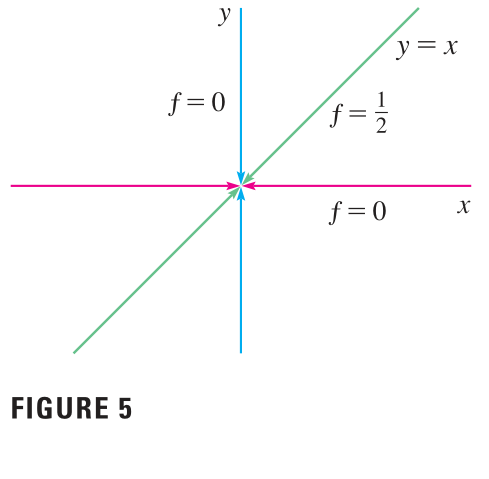
\includegraphics[width = 5 cm]{./images/lim3g2.png} 
      \end{center}
    \end{minipage}
  \begin{minipage}[]{0.6\linewidth}
    $\square$ If $y = 0$, then $f(x,0) = 0/ x^2 $
    \begin{center}
      $f(x,y) \to 0 \quad \text{as} \quad (x,y) \to (0,0)$ along the $x$-axis
    \end{center}
    $\square$ If $x = 0$, then $f(0,y) = -/ y^2 = 0$, so 
    \begin{center}
      $f(x,y) \to 0 \quad \text{as} \quad (x,y) \to (0,0)$ along the $y$-axis
    \end{center}
  \end{minipage}
Although we have obtained identical limits along the axes, that does not show the answer is 0.  \\
$\square$ Let's approach $(0,0)$ along another line, say $y = x$. For all $x \ne 0$,
\[f(x,x) = \frac{x^2 }{x^2 + x^2 } = \frac{1}{2}\]
Therefore $\quad f(x,y) \to \frac{1 }{2 } \quad \text{as} \quad (x,y) \to (0,0)$  along $y = x$. The given limit \textbf{does not exist}. 

The ridge that occurs above the line $y = x$ correspond to the fact that $f(x,y) = \frac{1 }{2 }$ for all points $(x,y)$ on that line \textbf{except the origin}.
\begin{center}
  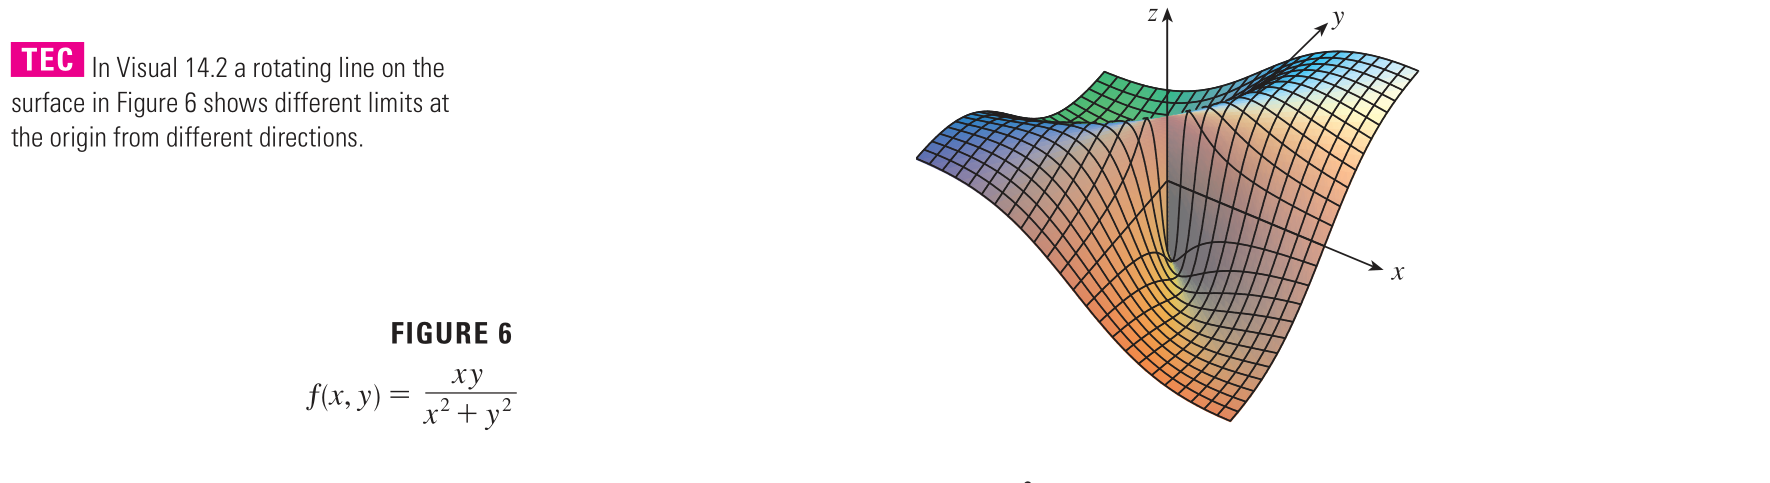
\includegraphics[width = \linewidth]{./images/limeg2.png} 
\end{center}
{\fontfamily{lmtt}\selectfont \textbf{\textcolor{blue5}{EXAMPLE.}}} Find the limit.
\[\lim_{(x,y) \to (0,0)} \frac{x y^2 }{x^2 + y^4}\]
Let's approach along any nonvertical line through the origin. Then $y = mx$, where $m$ is the slope, then
\[f(x,y) = f(x, mx) = \frac{x(mx)^2}{x^2 + (mx)^4} = \frac{m^2 x^3}{x^2 + m^4 x^4} = \frac{m^2 x}{1 + m^4 x^2}\]
So $\quad f(x,y) \to 0 \quad \text{as} \quad (x,y) \to (0,0)$ along $y = mx$.\\
Thus $f$ has the same limiting value along \textit{every nonvertical line} through the origin. But that does not show that the answer is 0, if we now let $(x,y) \to (0,0)$ along the parabola $x = y^2$, we have 
\[f(x,y) = f(y^2, y) = \frac{y^2 \dot y^2 }{(y^2 )^2 + y^4} = \frac{y^4}{2y^4} = \frac{1 }{2 }\]
Hence, the limit \textbf{does not exist}.

\begin{mdframed}
 \textbf{What limits that do exist then?} 

 The limit of a \textbf{sum} the sum of the limits, so does a \textbf{product}. These equations are true.
 \begin{align*}
   \lim_{(x,y) \to (a,b)} x = a & \quad & \lim_{(x,y) \to (a,b)} y = b & \quad & \lim_{(x,y) \to (a,b)} c = c 
 \end{align*}
 The Squeeze Theorem also holds.
\end{mdframed}
{\fontfamily{lmtt}\selectfont \textbf{\textcolor{blue5}{EXAMPLE.}}} Find the limit.
\[\lim_{(x,y) \to (0,0)}\frac{3 x^2 y }{x^2 + y^2 }\]
$\square$ As the previous example, we see that the limit along any line through the origin is 0. Plus, the limits along the parabolas $y = x^2$ and $x = y^2$ are also 0, so we suspect the limit exist and equal to 0.\\
$\square$ Let $\varepsilon > 0$. We want to find $\delta > 0 $ such that 
\[\text{if } \quad 0 < \sqrt{x^2 + y^2 } < \delta \quad \text{ then } \quad \abs{ \frac{3x^2 y }{x^2 + y^2 } - 0  } < \varepsilon \]
That is, 
\[\text{if } \quad 0 < \sqrt{x^2 + y^2 } < \delta \quad   \text{ then } \quad  \frac{3x^2 |y| }{x^2 + y^2   } < \varepsilon \]
Since $ x^2 \le x^2 + y^2 $, so $x^2 / (x^2 + y^2 ) \le 1$ and therefore 
\[\frac{3 x^2 |y| }{x^2 + y^2 } \le 3 |y| = 3 \sqrt{y^2 } \le 3 \sqrt{x^2 + y^2 } < 3 \delta \]
Thus we choose $\delta = \varepsilon / 3 $ and let $0 < \sqrt{x^2 + y^2 } < \delta $, then 
\[\frac{3 x^2 |y| }{x^2 + y^2 } \le 3 \sqrt{x^2 + y^2 } < 3 \delta = 3 \left(\frac{\varepsilon }{3 }\right) = \varepsilon   \]
Hence, by the \textbf{Definition: Limit}, 
\[\lim_{(x,y) \to (0,0)} \frac{3 x^2 y }{x^2 + y^2 } = 0 \]

\subsection*{{\fontfamily{lmss}\selectfont \underline{Continuity}}}
Limits of \textit{continuous} functions is easy evaluated by direct substitution.
\begin{Def}[Continuous]
  A function $f$ is \textbf{continuous at $(a,b)$} if 
  \[\lim_{(x,y) \to (a,b)} f(x,y) = f(a,b)\]
  We say $f$ is \textbf{continuous on $D$} if $f$ is continuous at \textit{every} point $(a,b)$ in $D$.
\end{Def}
\end{document}
